\section{Comparison of 1D and 2D QCD k-factors}
\label{sec:1d_vs_2d_kfac}

In this appendix, several distributions such as recoil, $\mjj$ and $\detajj$ are compared for two cases in the single muon
control region:

\begin{itemize}
    \item Plots with 1D k-factors applied: Function of gen-boson pt
    \item Plots with 2D k-factors applied: Function of gen-boson pt and $\mjj$
\end{itemize}

Both k-factors are derived from samples in which the VBF selections are applied at the gen level. 1D k-factor is a function of
generator level vector boson $\pt$, whereas 2D k-factor is a function of both generator level boson $\pt$ and $\mjj$. 
The distributions are shown in the following pages. 

Fig.~\ref{fig:recoil_2017} shows the comparison of the recoil distribution 
with 2017 samples, while Fig.~\ref{fig:recoil_2018} shows the same comparison with 2018 samples. 
Fig.~\ref{fig:mjj_2017} shows the comparison of the $\mjj$ distribution 
with 2017 samples, while Fig.~\ref{fig:mjj_2018} shows the same comparison with 2018 samples. 
Fig.~\ref{fig:detajj_2017} shows the comparison of the $\detajj$ distribution 
with 2017 samples, while Fig.~\ref{fig:detajj_2018} shows the same comparison with 2018 samples. 
Fig.~\ref{fig:muon_pt_2017} shows the comparison of the muon $\pt$ distribution 
with 2017 samples, while Fig.~\ref{fig:muon_pt_2018} shows the same comparison with 2018 samples. 
Fig.~\ref{fig:muon_eta_2017} shows the comparison of the muon $\eta$ distribution 
with 2017 samples, while Fig.~\ref{fig:muon_eta_2018} shows the same comparison with 2018 samples. 

\begin{figure}
    \begin{center}
        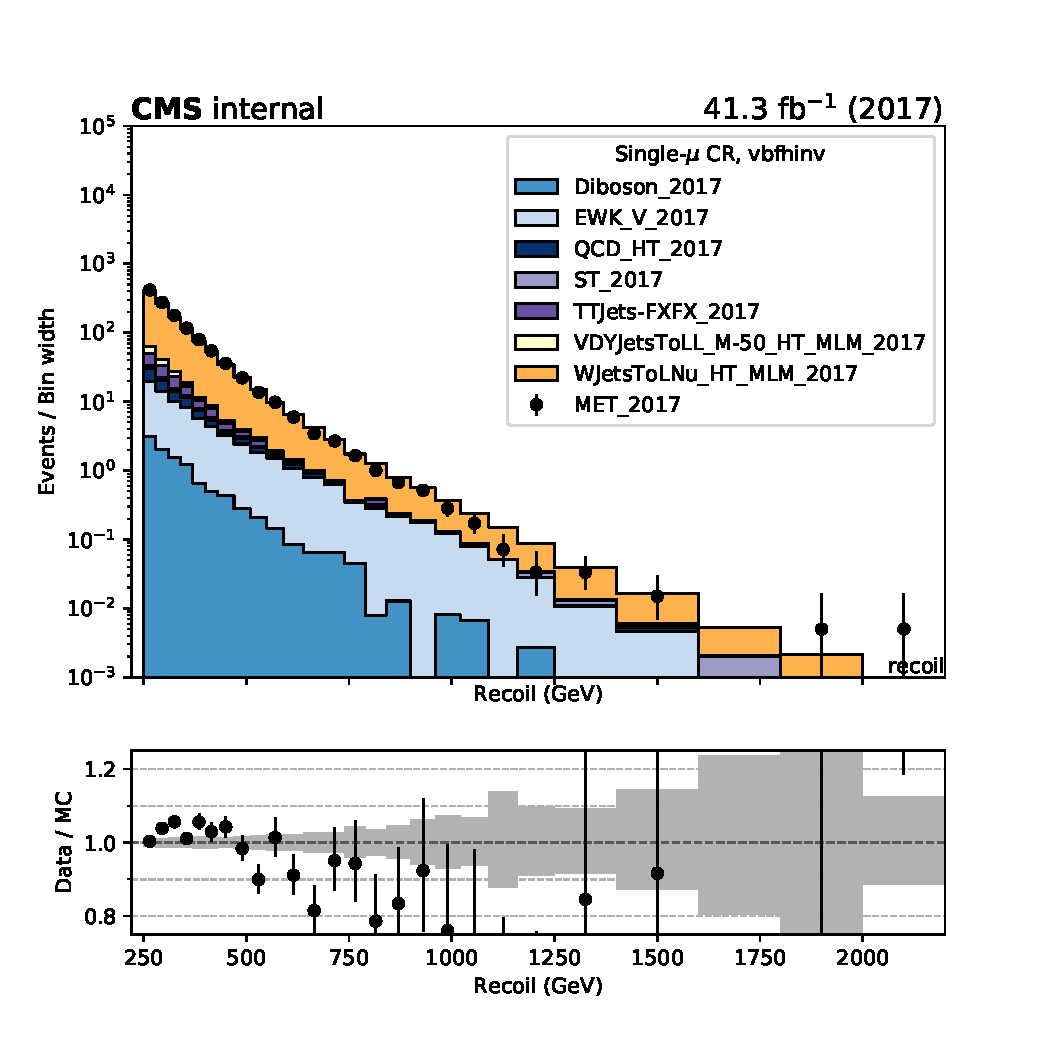
\includegraphics[width=0.49\textwidth]{fig/datamc/cr_1m_vbf/cr_1m_vbf_recoil_losf_2017.pdf}
        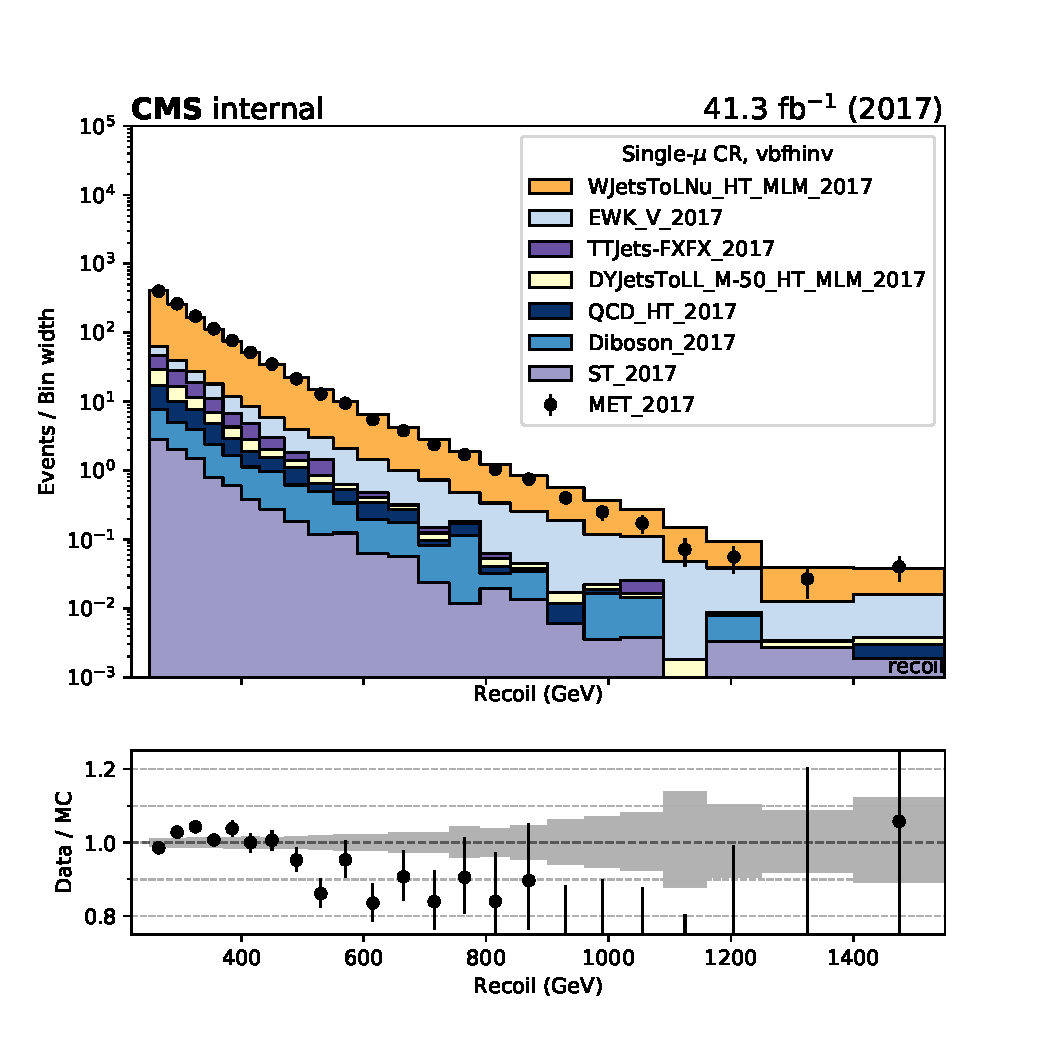
\includegraphics[width=0.49\textwidth]{fig/datamc_2dkfac/cr_1m_vbf/cr_1m_vbf_recoil_losf_2017.pdf} 
        \caption{The recoil distribution in the single muon CR for the case in which 1D k-factors are used (left), 
        compared to the case in which 2D k-factors are used (right), using 2017 samples.}
        \label{fig:recoil_2017}
    \end{center}
\end{figure}

\begin{figure}
    \begin{center}
        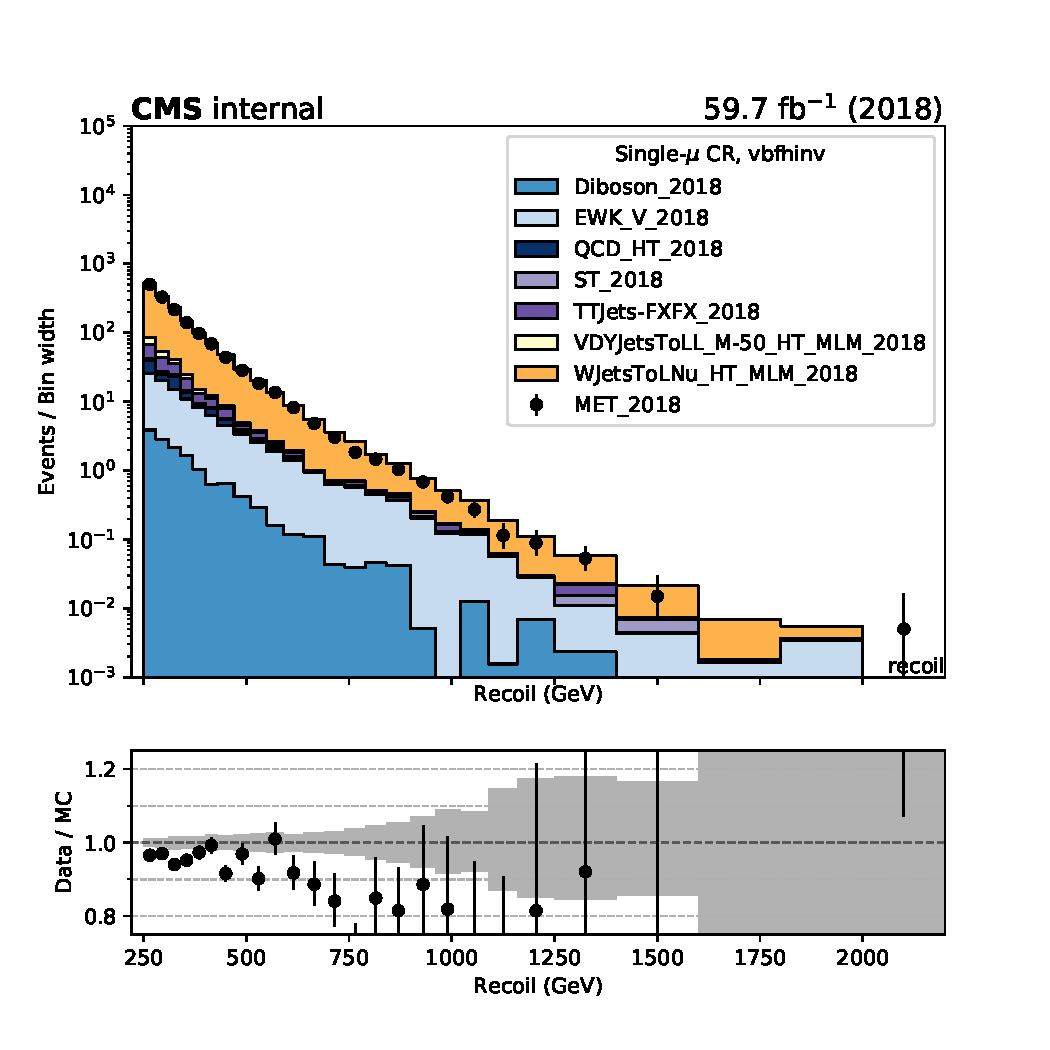
\includegraphics[width=0.49\textwidth]{fig/datamc/cr_1m_vbf/cr_1m_vbf_recoil_losf_2018.pdf}
        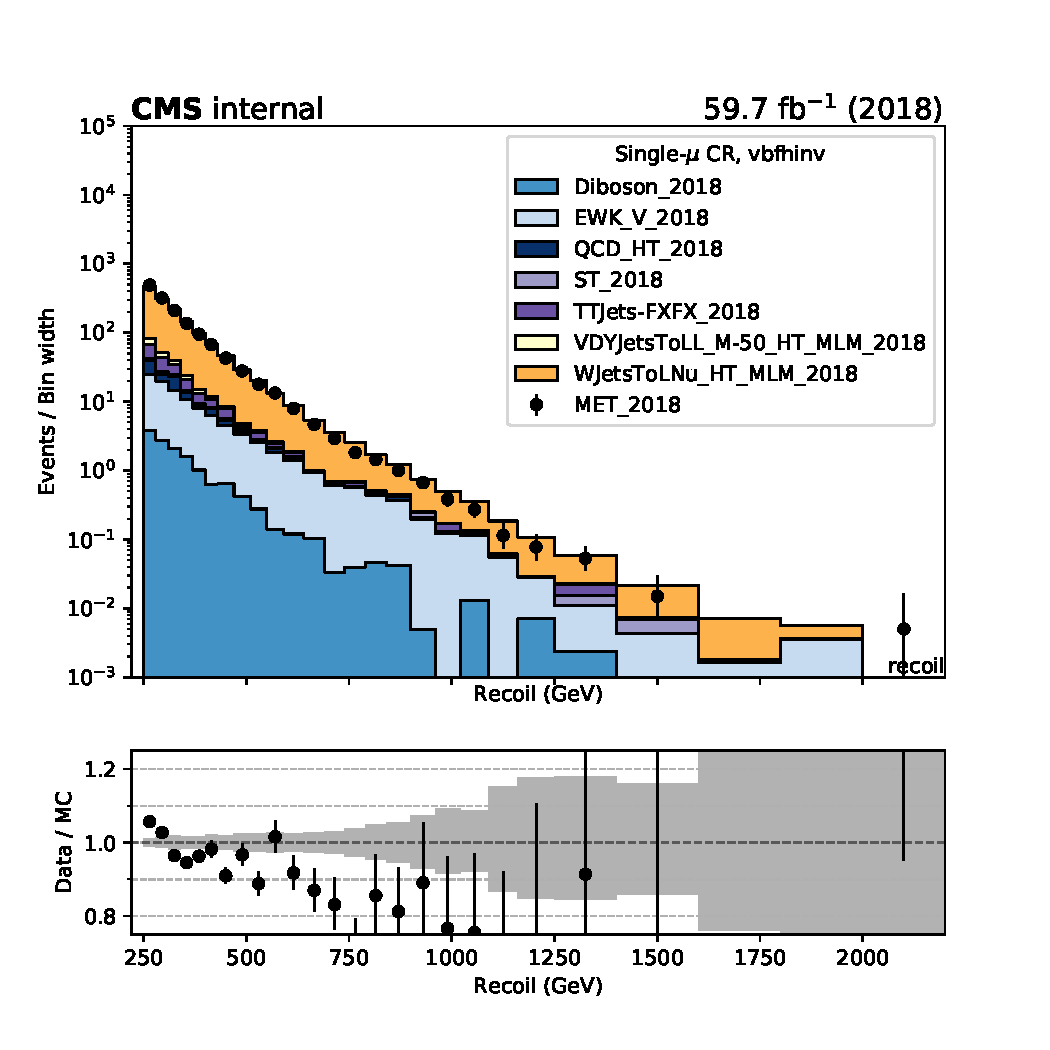
\includegraphics[width=0.49\textwidth]{fig/datamc_2dkfac/cr_1m_vbf/cr_1m_vbf_recoil_losf_2018.pdf} 
        \caption{The recoil distribution in the single muon CR for the case in which 1D k-factors are used (left), 
        compared to the case in which 2D k-factors are used (right), using 2018 samples.}
        \label{fig:recoil_2018}
    \end{center}
\end{figure}

\begin{figure}
    \begin{center}
        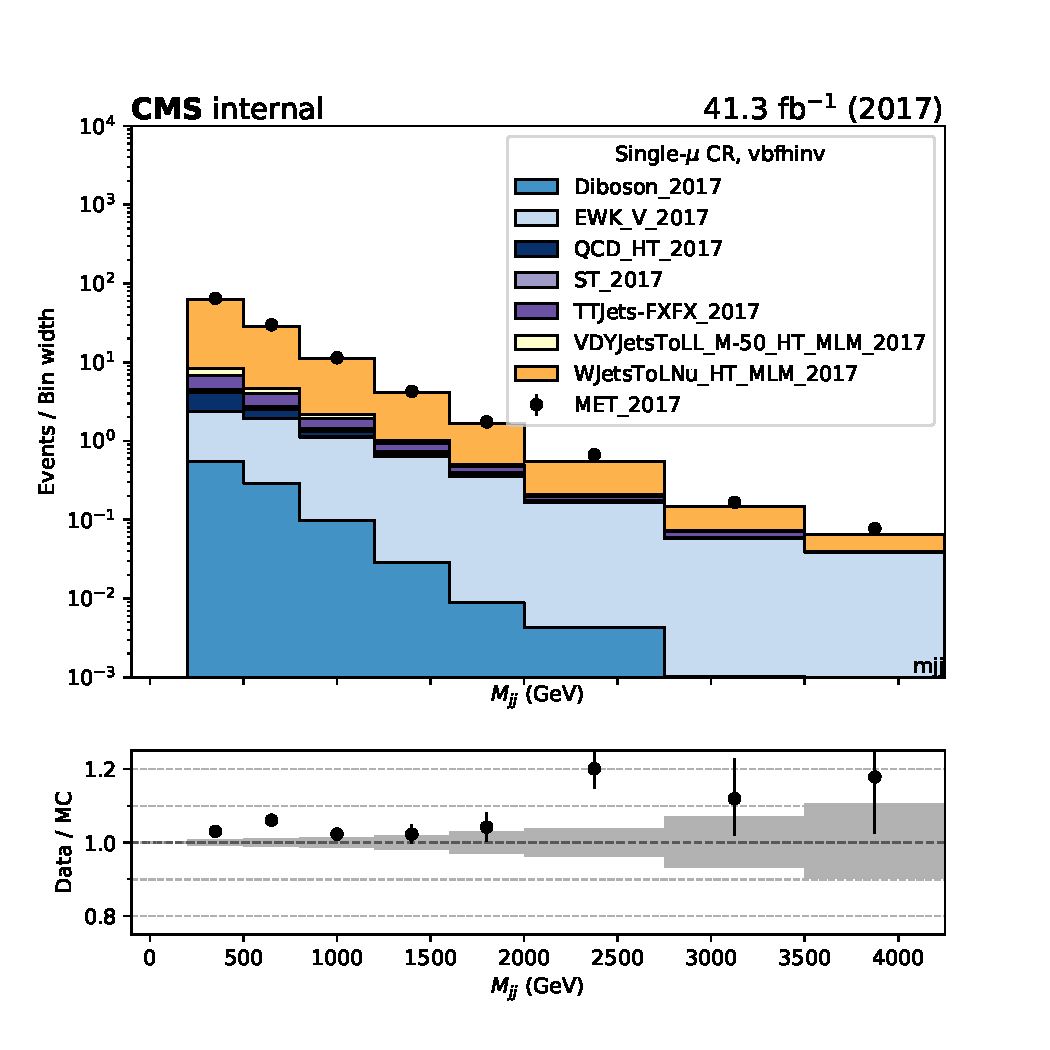
\includegraphics[width=0.49\textwidth]{fig/datamc/cr_1m_vbf/cr_1m_vbf_mjj_losf_2017.pdf}
        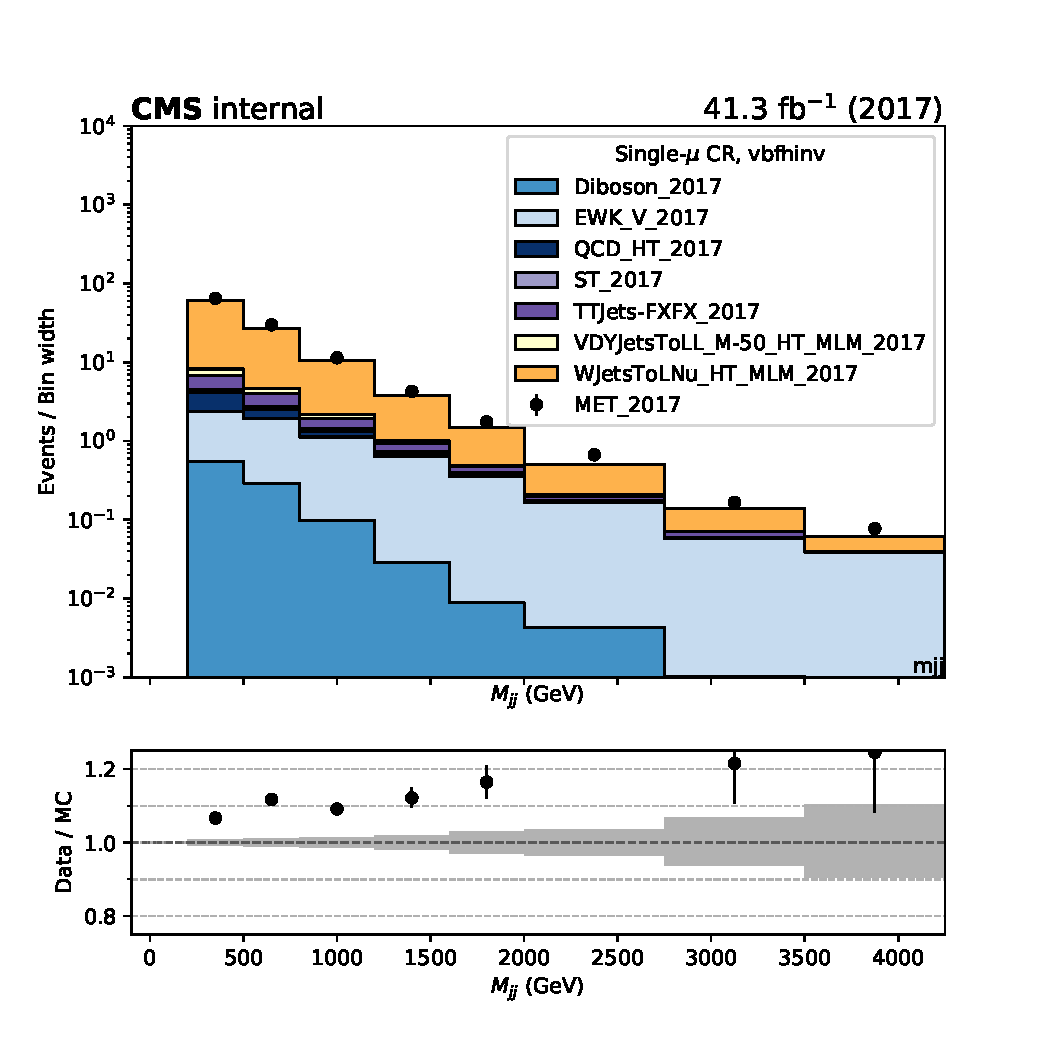
\includegraphics[width=0.49\textwidth]{fig/datamc_2dkfac/cr_1m_vbf/cr_1m_vbf_mjj_losf_2017.pdf} 
        \caption{The $\mjj$ distribution in the single muon CR for the case in which 1D k-factors are used (left), 
        compared to the case in which 2D k-factors are used (right), using 2017 samples.}
        \label{fig:mjj_2017}
    \end{center}
\end{figure}

\begin{figure}
    \begin{center}
        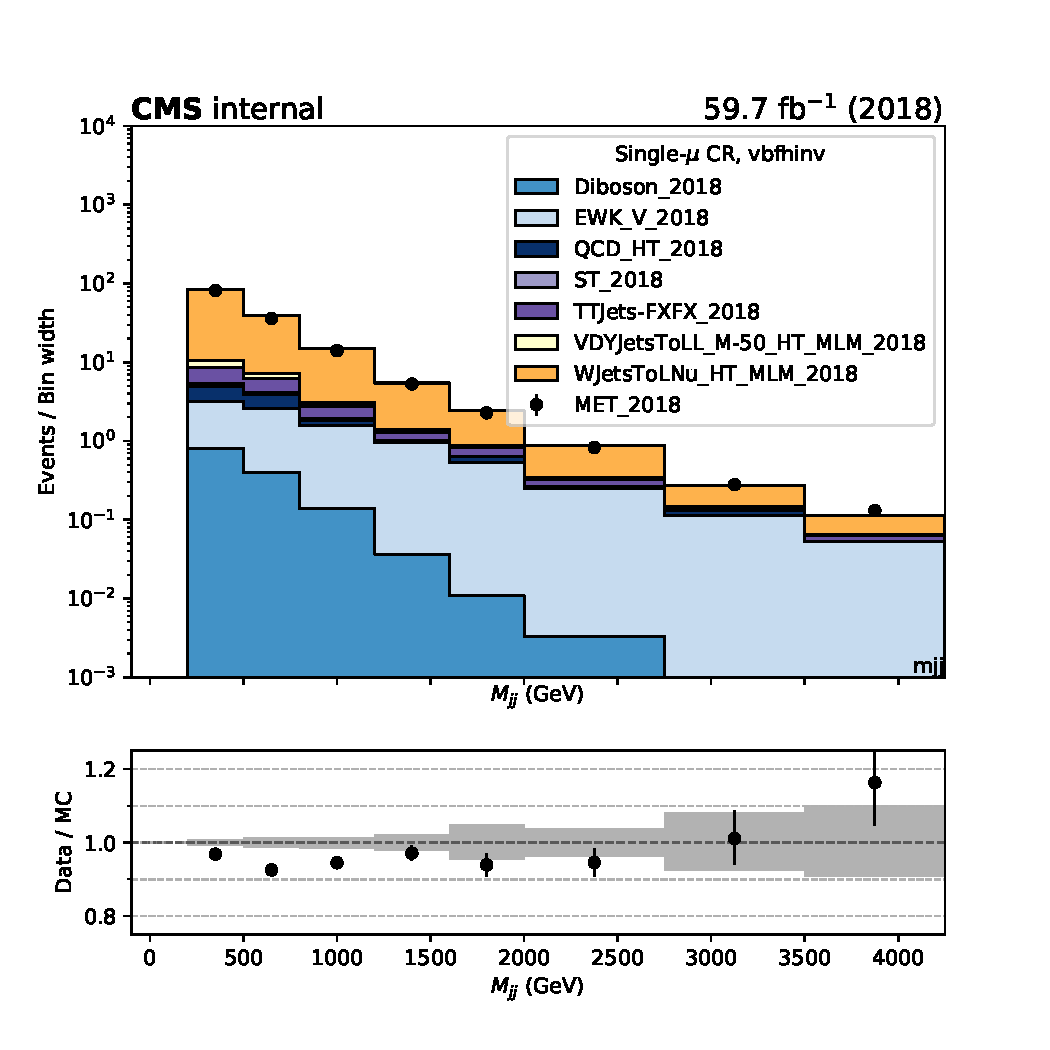
\includegraphics[width=0.49\textwidth]{fig/datamc/cr_1m_vbf/cr_1m_vbf_mjj_losf_2018.pdf}
        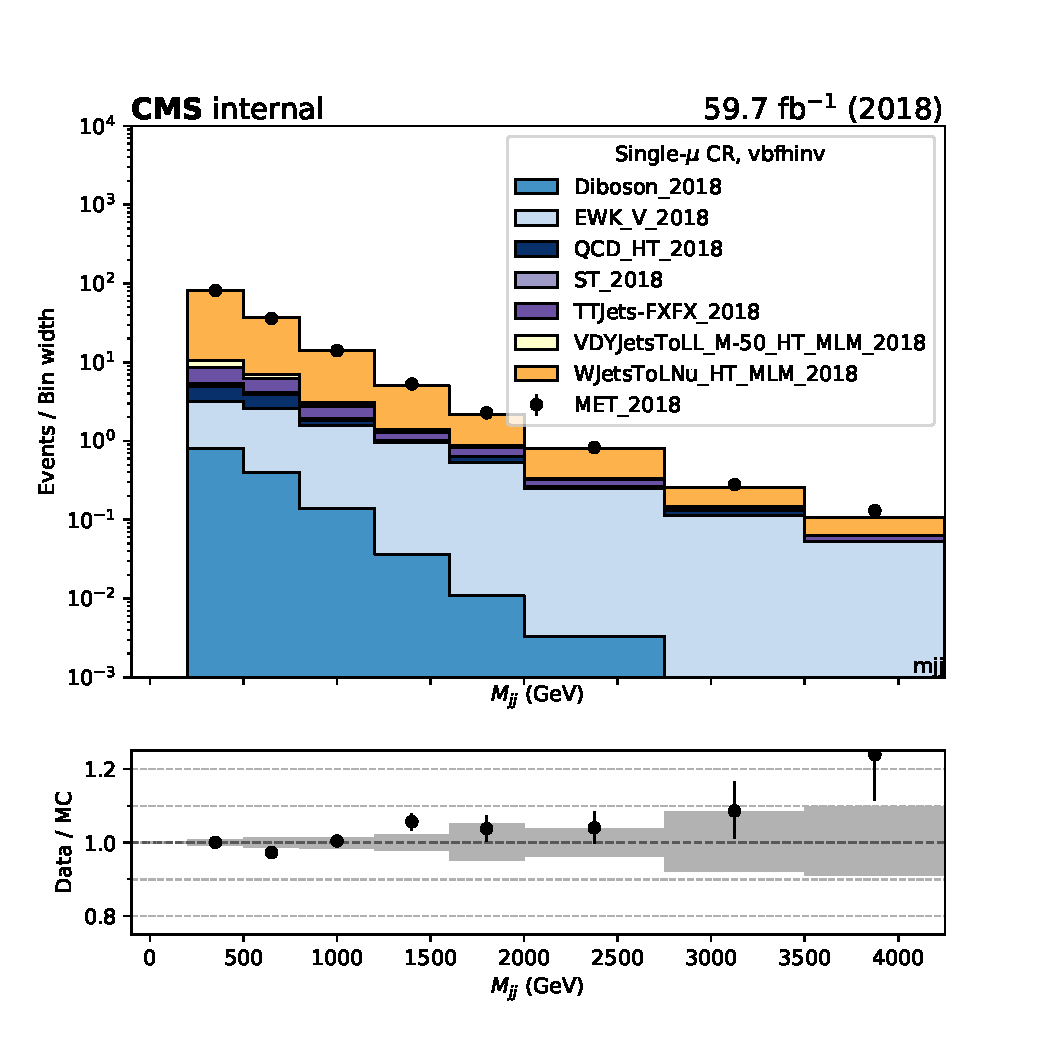
\includegraphics[width=0.49\textwidth]{fig/datamc_2dkfac/cr_1m_vbf/cr_1m_vbf_mjj_losf_2018.pdf} 
        \caption{The $\mjj$ distribution in the single muon CR for the case in which 1D k-factors are used (left), 
        compared to the case in which 2D k-factors are used (right), using 2018 samples.}
        \label{fig:mjj_2018}
    \end{center}
\end{figure}

\begin{figure}
    \begin{center}
        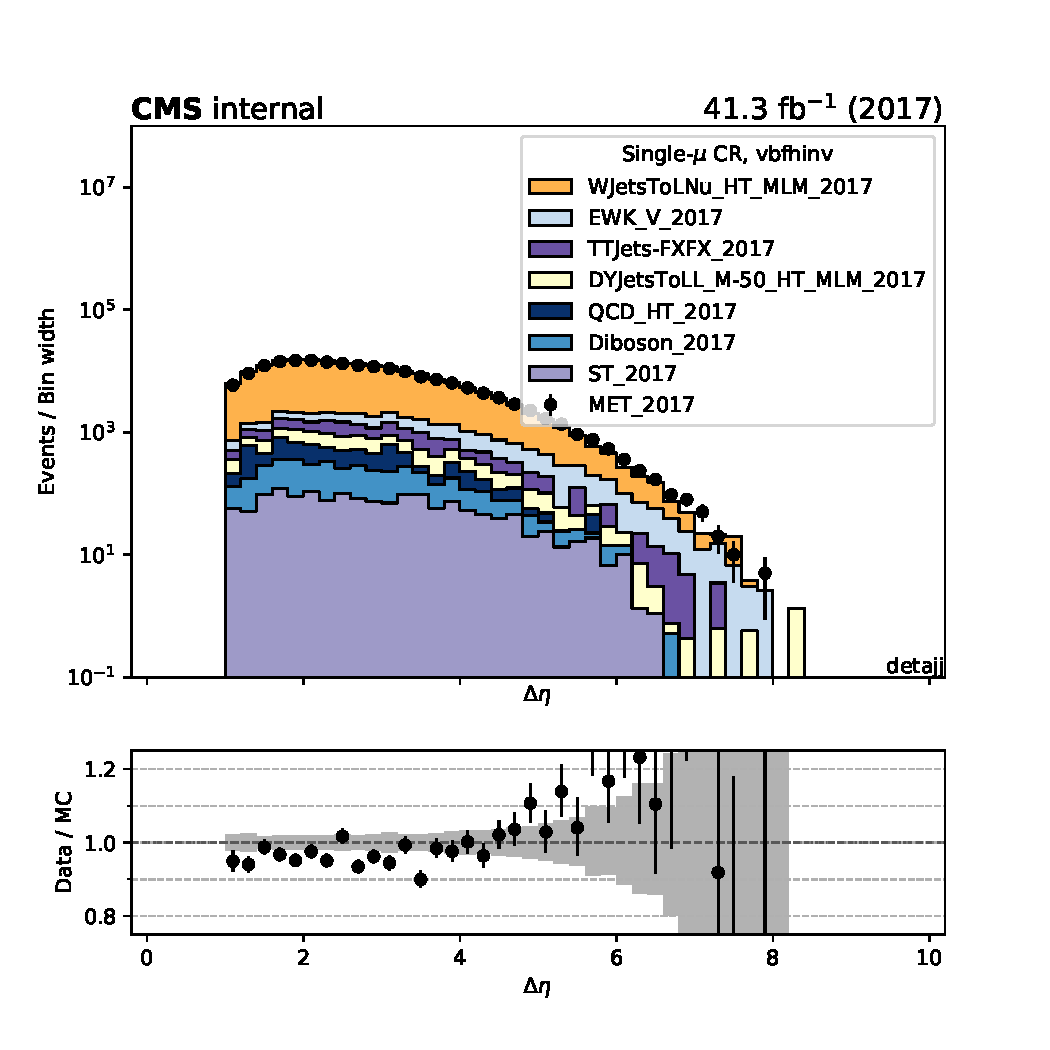
\includegraphics[width=0.49\textwidth]{fig/datamc/cr_1m_vbf/cr_1m_vbf_detajj_losf_2017.pdf}
        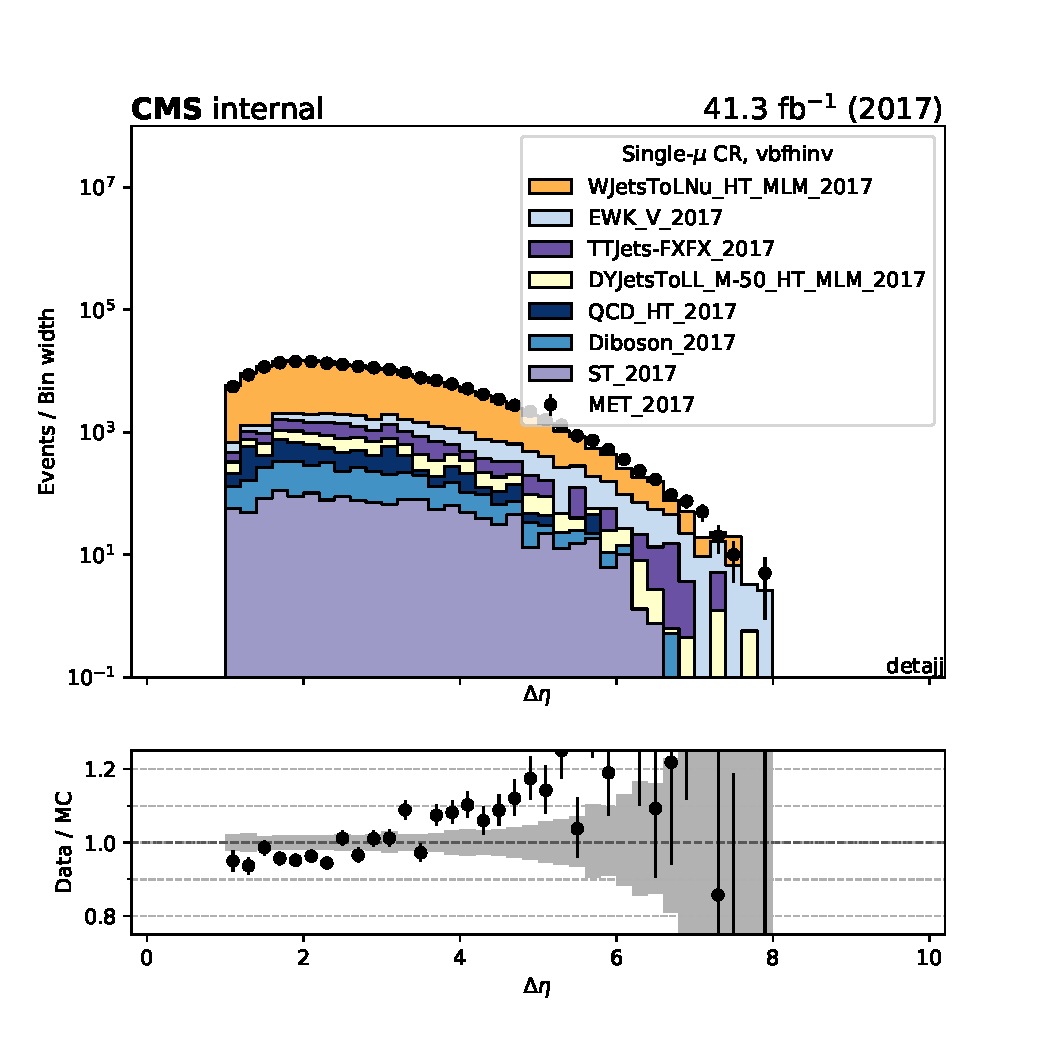
\includegraphics[width=0.49\textwidth]{fig/datamc_2dkfac/cr_1m_vbf/cr_1m_vbf_detajj_losf_2017.pdf} 
        \caption{The $\detajj$ distribution in the single muon CR for the case in which 1D k-factors are used (left), 
        compared to the case in which 2D k-factors are used (right), using 2017 samples.}
        \label{fig:detajj_2017}
    \end{center}
\end{figure}

\begin{figure}
    \begin{center}
        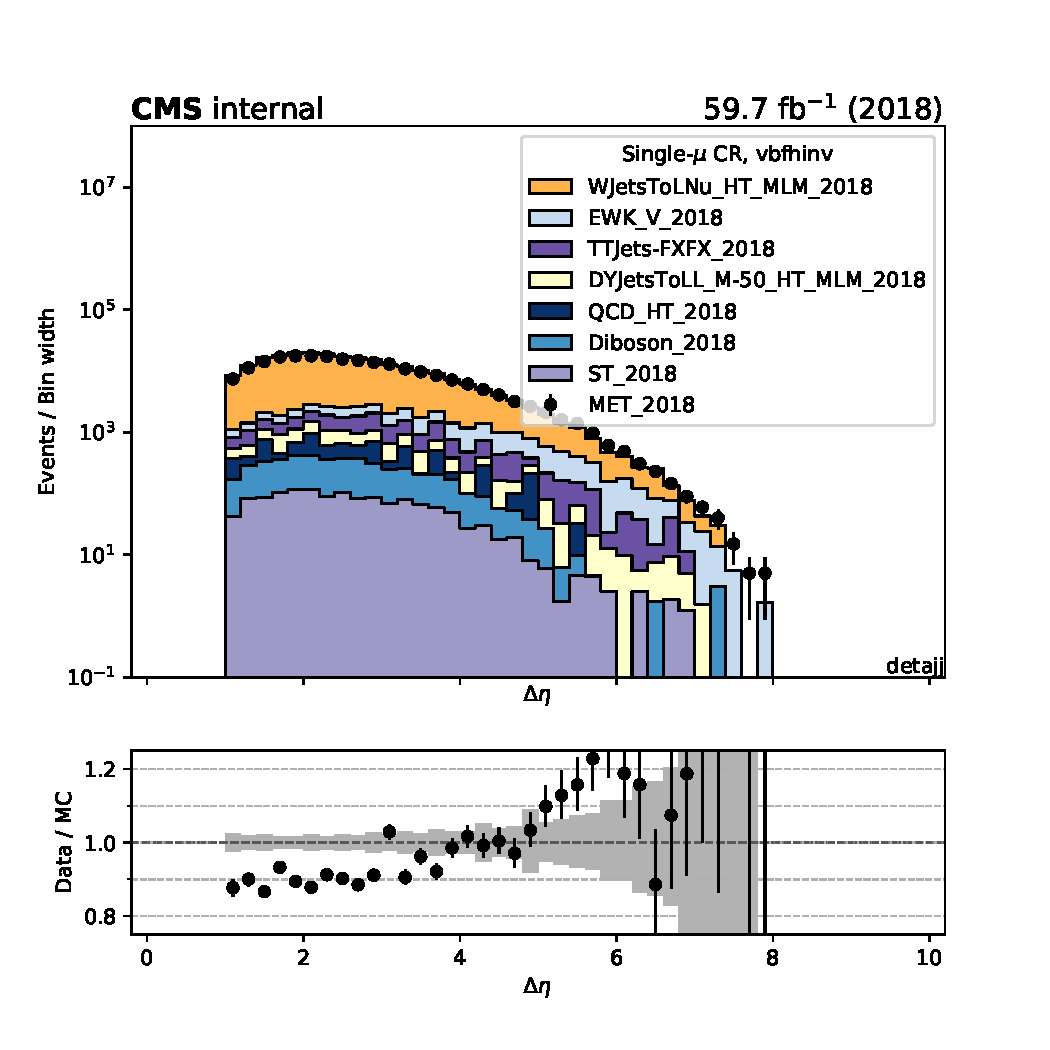
\includegraphics[width=0.49\textwidth]{fig/datamc/cr_1m_vbf/cr_1m_vbf_detajj_losf_2018.pdf}
        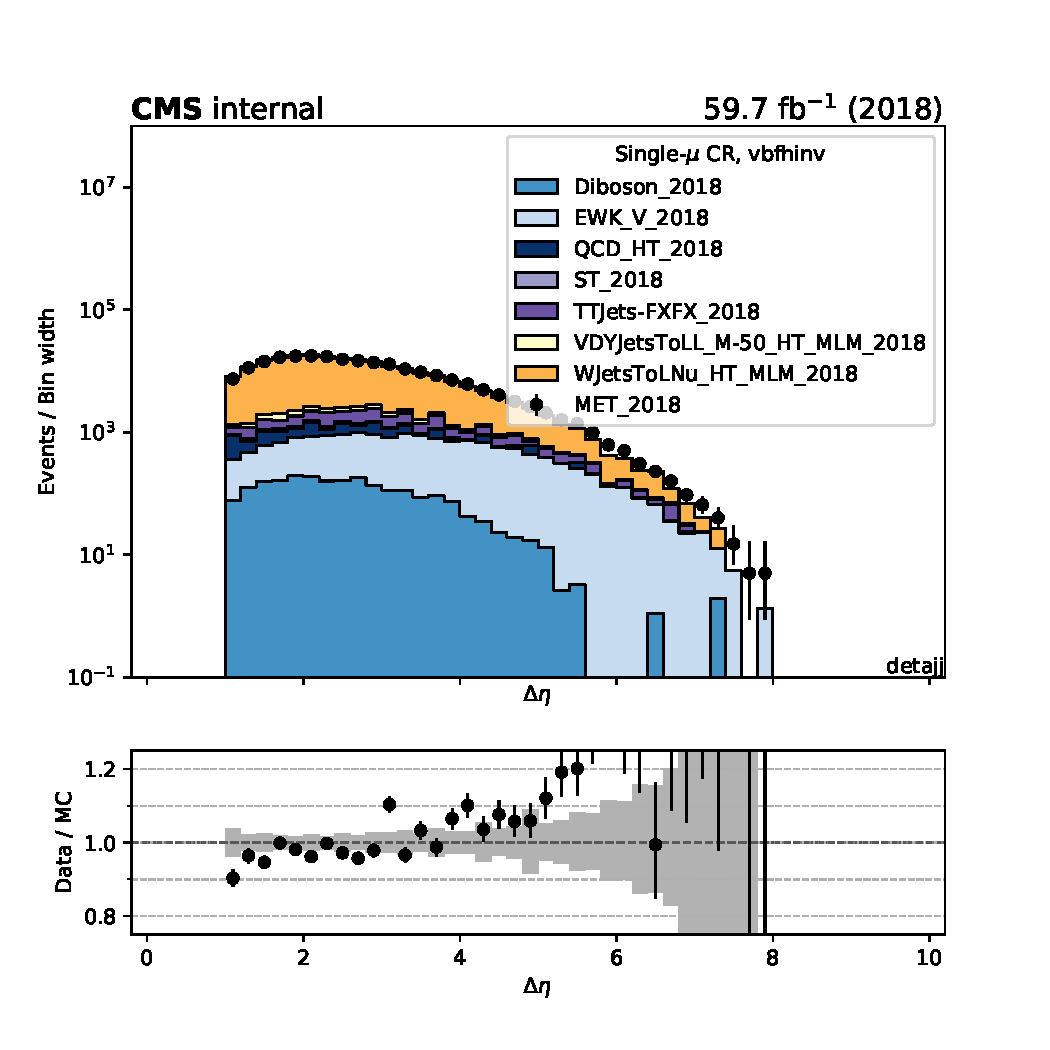
\includegraphics[width=0.49\textwidth]{fig/datamc_2dkfac/cr_1m_vbf/cr_1m_vbf_detajj_losf_2018.pdf} 
        \caption{The $\detajj$ distribution in the single muon CR for the case in which 1D k-factors are used (left), 
        compared to the case in which 2D k-factors are used (right), using 2018 samples.}
        \label{fig:detajj_2018}
    \end{center}
\end{figure}

\begin{figure}
    \begin{center}
        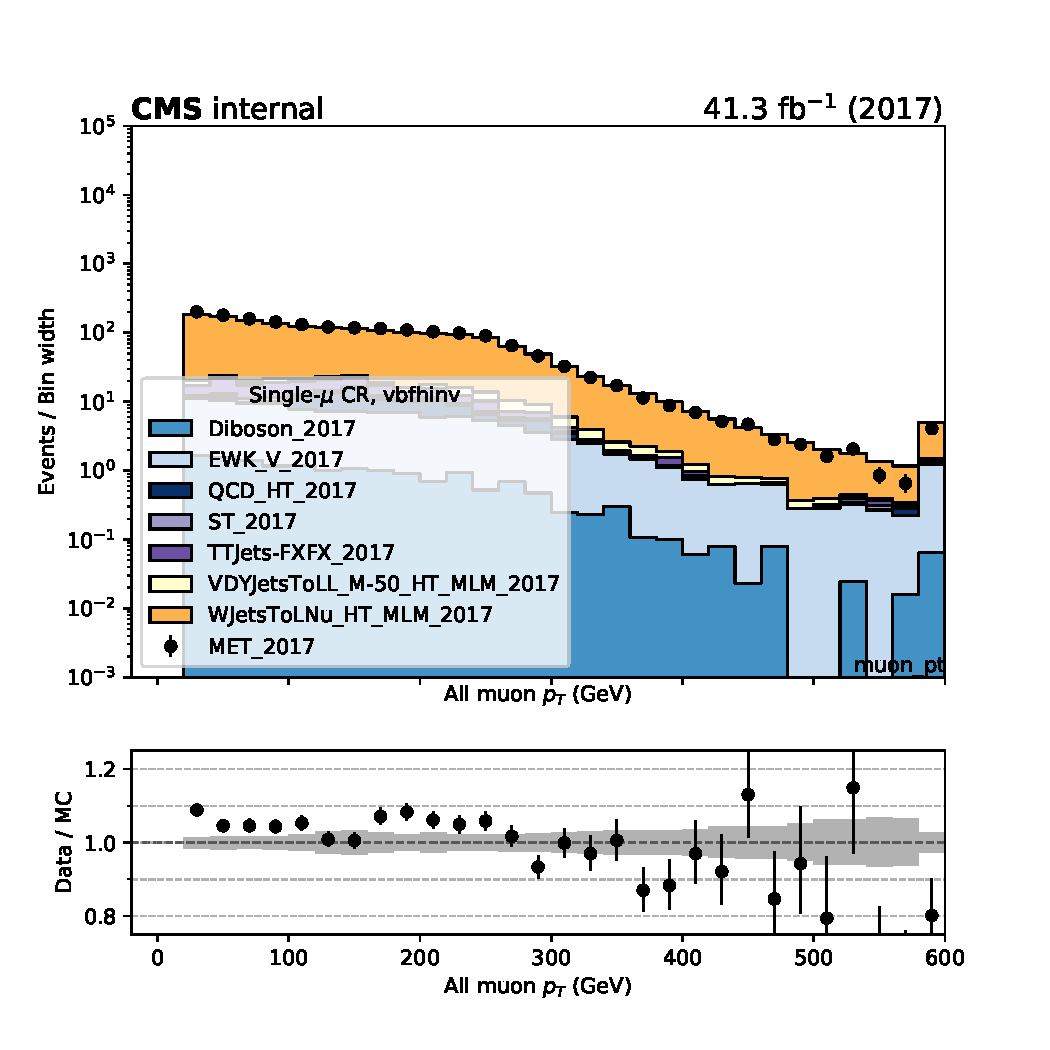
\includegraphics[width=0.49\textwidth]{fig/datamc/cr_1m_vbf/cr_1m_vbf_muon_pt_losf_2017.pdf}
        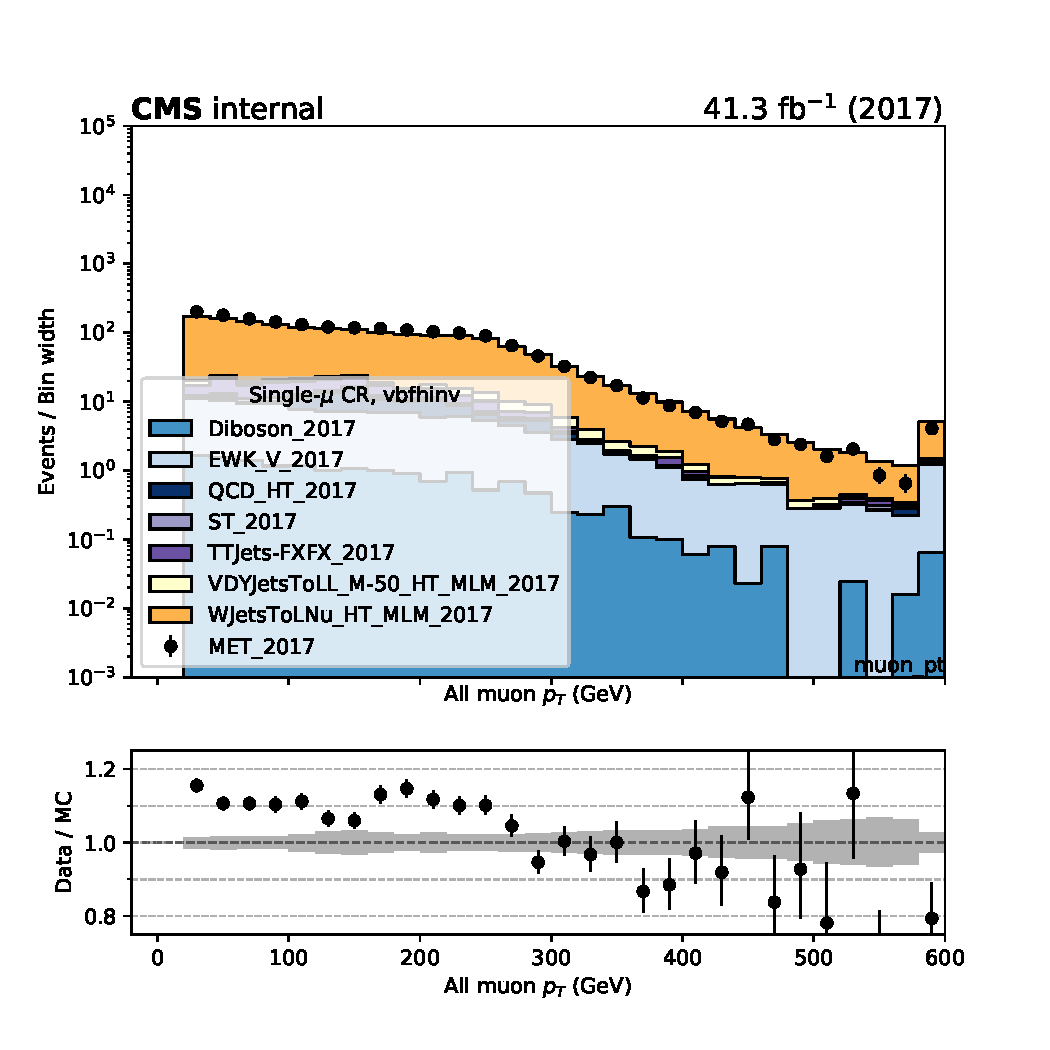
\includegraphics[width=0.49\textwidth]{fig/datamc_2dkfac/cr_1m_vbf/cr_1m_vbf_muon_pt_losf_2017.pdf} 
        \caption{The muon $\pt$ distribution in the single muon CR for the case in which 1D k-factors are used (left), 
        compared to the case in which 2D k-factors are used (right), using 2017 samples.}
        \label{fig:muon_pt_2017}
    \end{center}
\end{figure}

\begin{figure}
    \begin{center}
        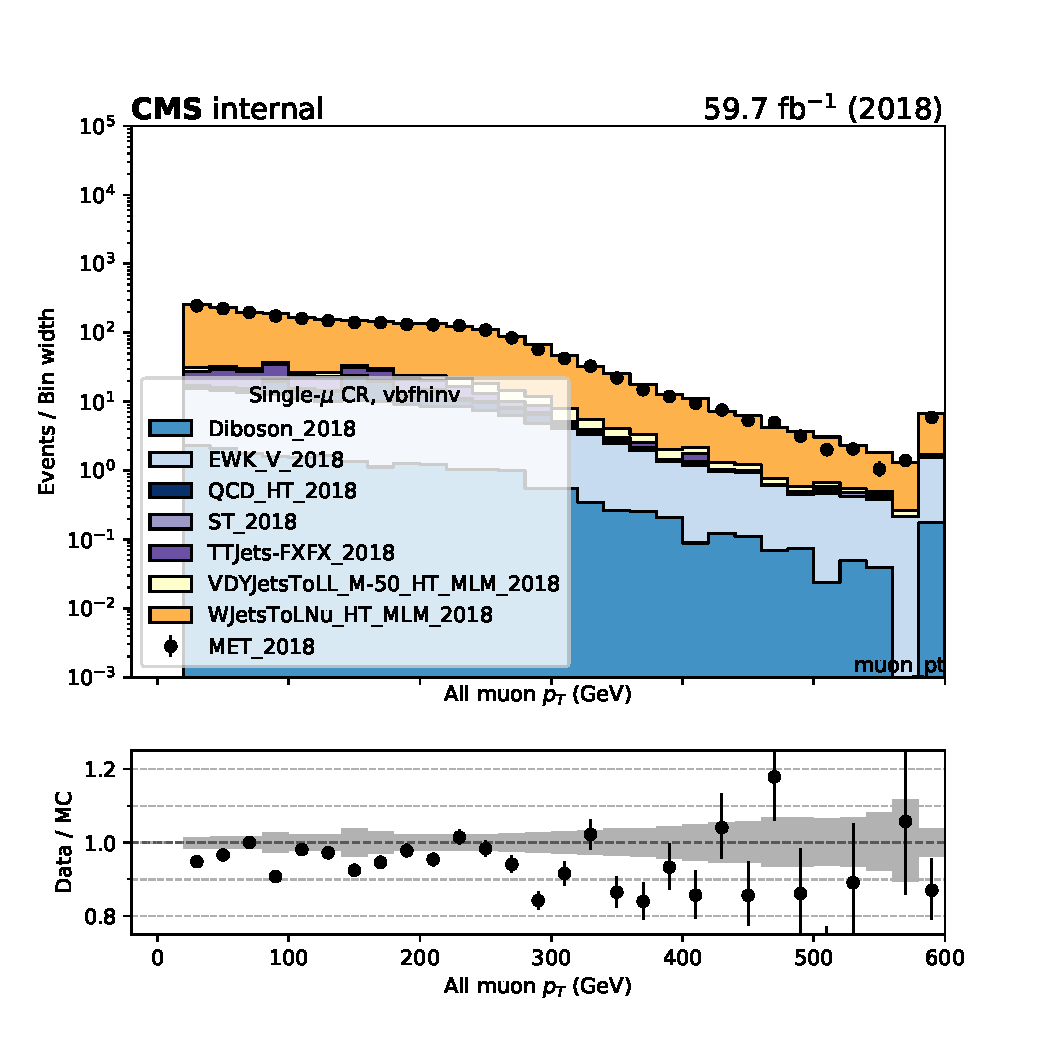
\includegraphics[width=0.49\textwidth]{fig/datamc/cr_1m_vbf/cr_1m_vbf_muon_pt_losf_2018.pdf}
        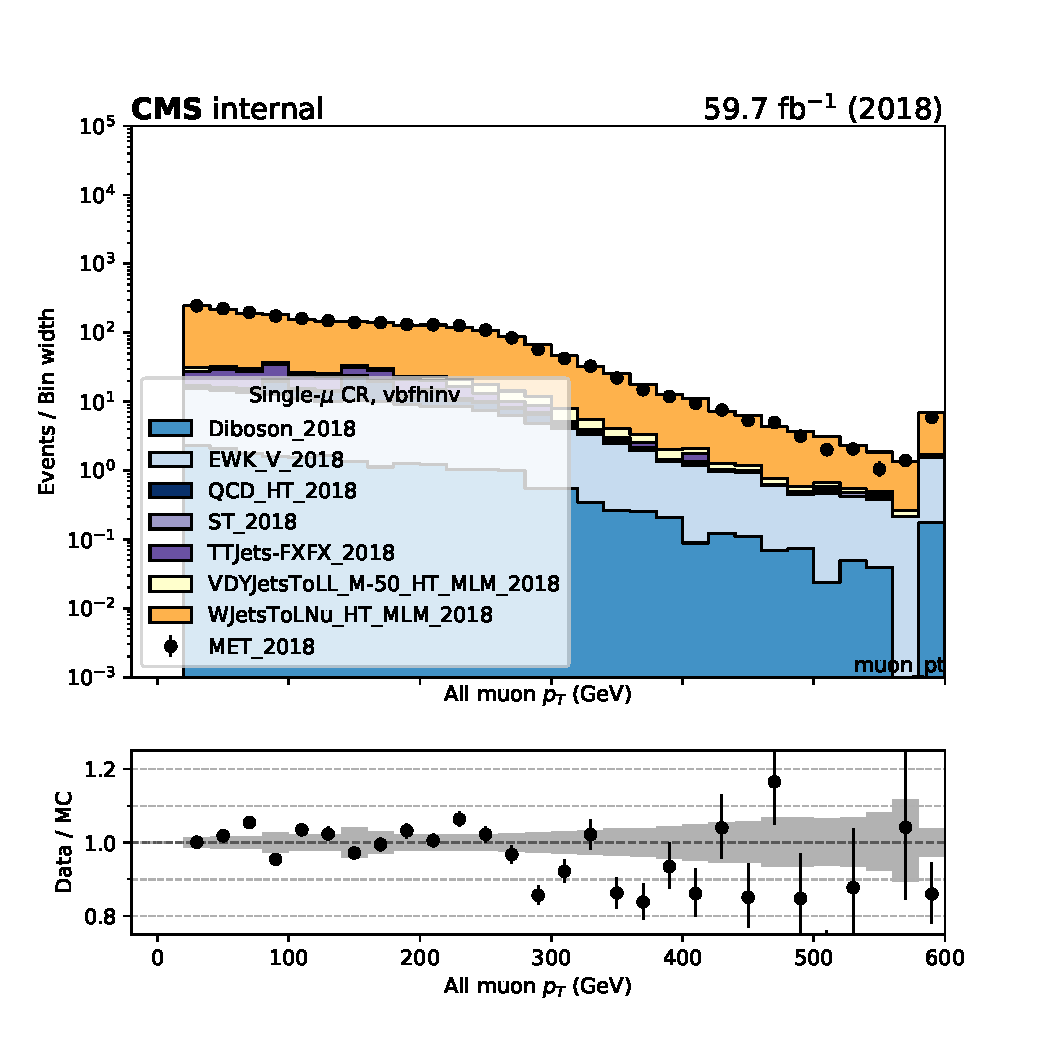
\includegraphics[width=0.49\textwidth]{fig/datamc_2dkfac/cr_1m_vbf/cr_1m_vbf_muon_pt_losf_2018.pdf} 
        \caption{The muon $\pt$ distribution in the single muon CR for the case in which 1D k-factors are used (left), 
        compared to the case in which 2D k-factors are used (right), using 2018 samples.}
        \label{fig:muon_pt_2018}
    \end{center}
\end{figure}

\begin{figure}
    \begin{center}
        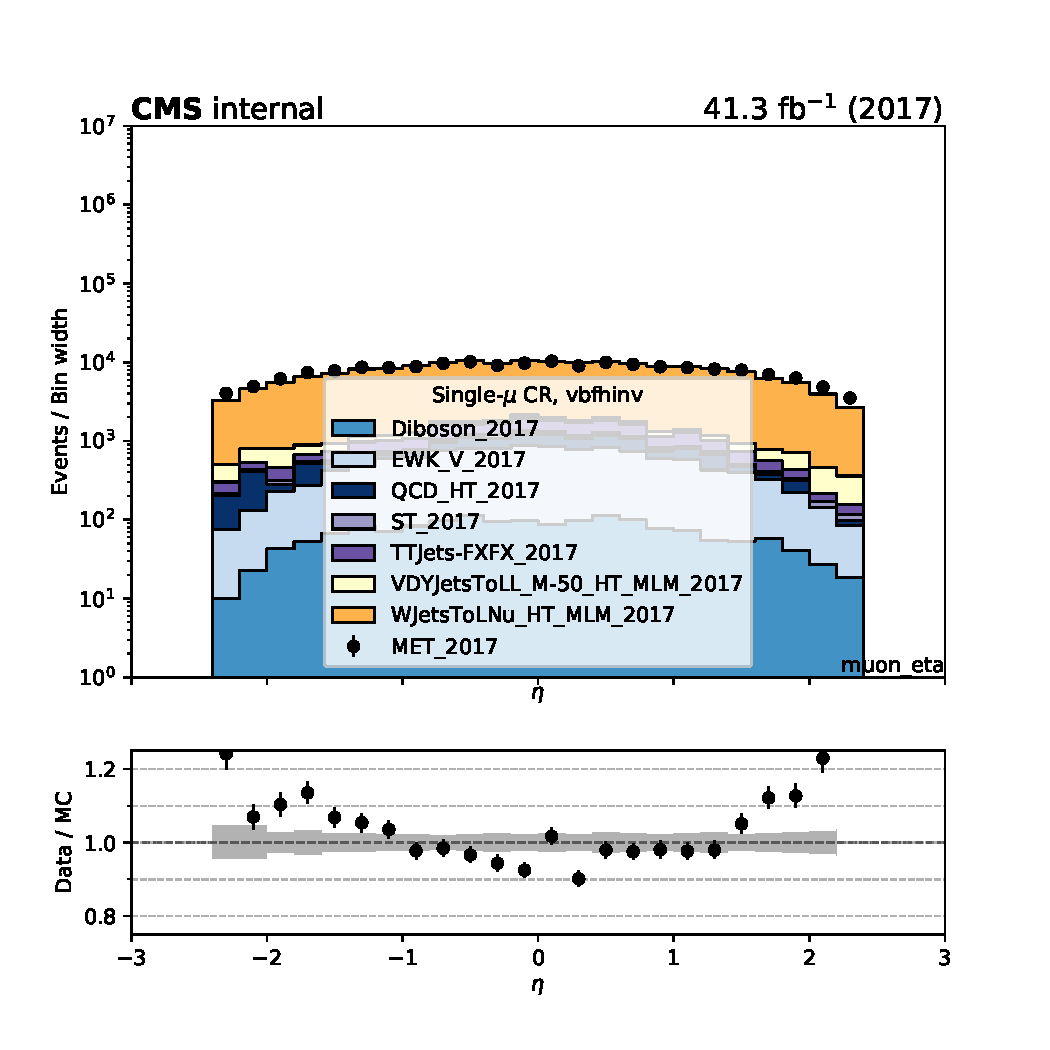
\includegraphics[width=0.49\textwidth]{fig/datamc/cr_1m_vbf/cr_1m_vbf_muon_eta_losf_2017.pdf}
        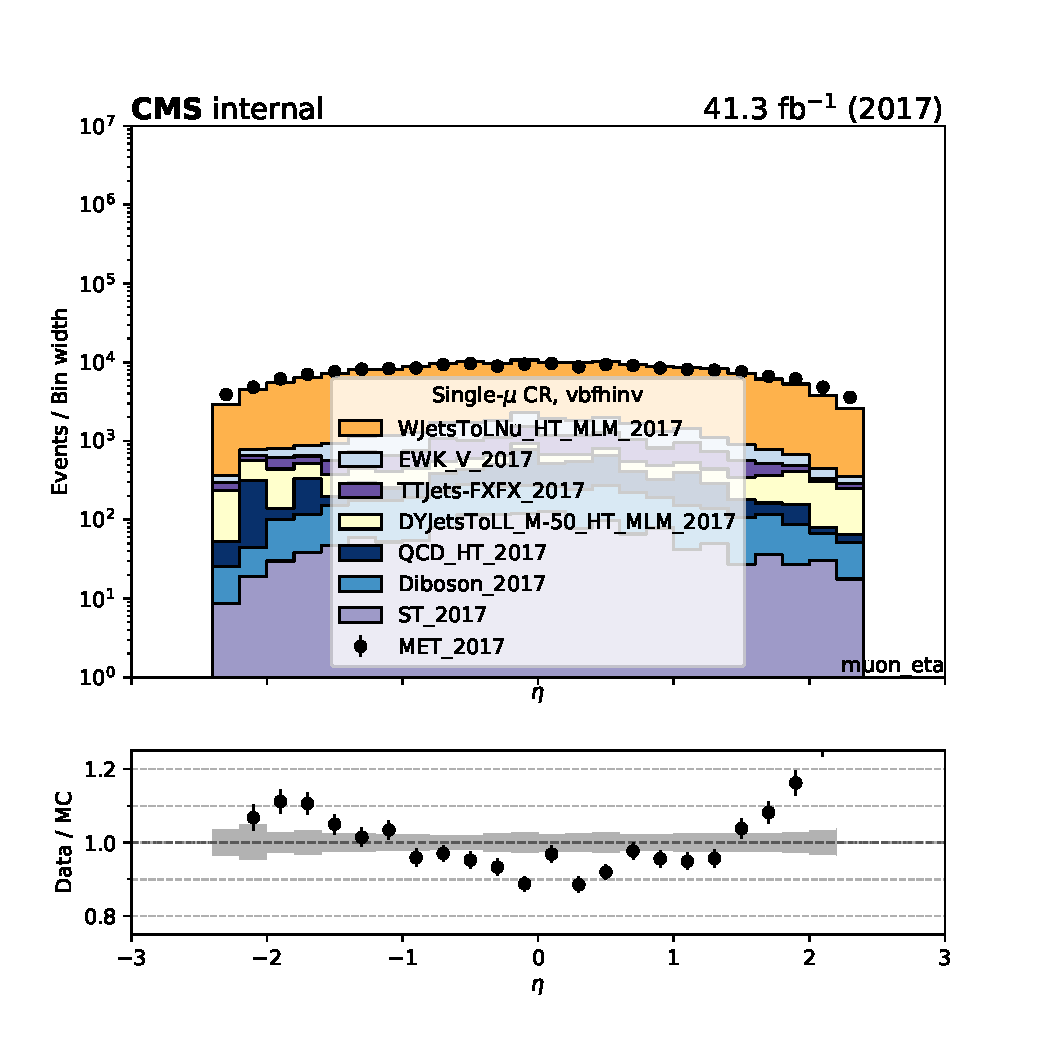
\includegraphics[width=0.49\textwidth]{fig/datamc_2dkfac/cr_1m_vbf/cr_1m_vbf_muon_eta_losf_2017.pdf} 
        \caption{The muon $\eta$ distribution in the single muon CR for the case in which 1D k-factors are used (left), 
        compared to the case in which 2D k-factors are used (right), using 2017 samples.}
        \label{fig:muon_eta_2017}
    \end{center}
\end{figure}

\begin{figure}
    \begin{center}
        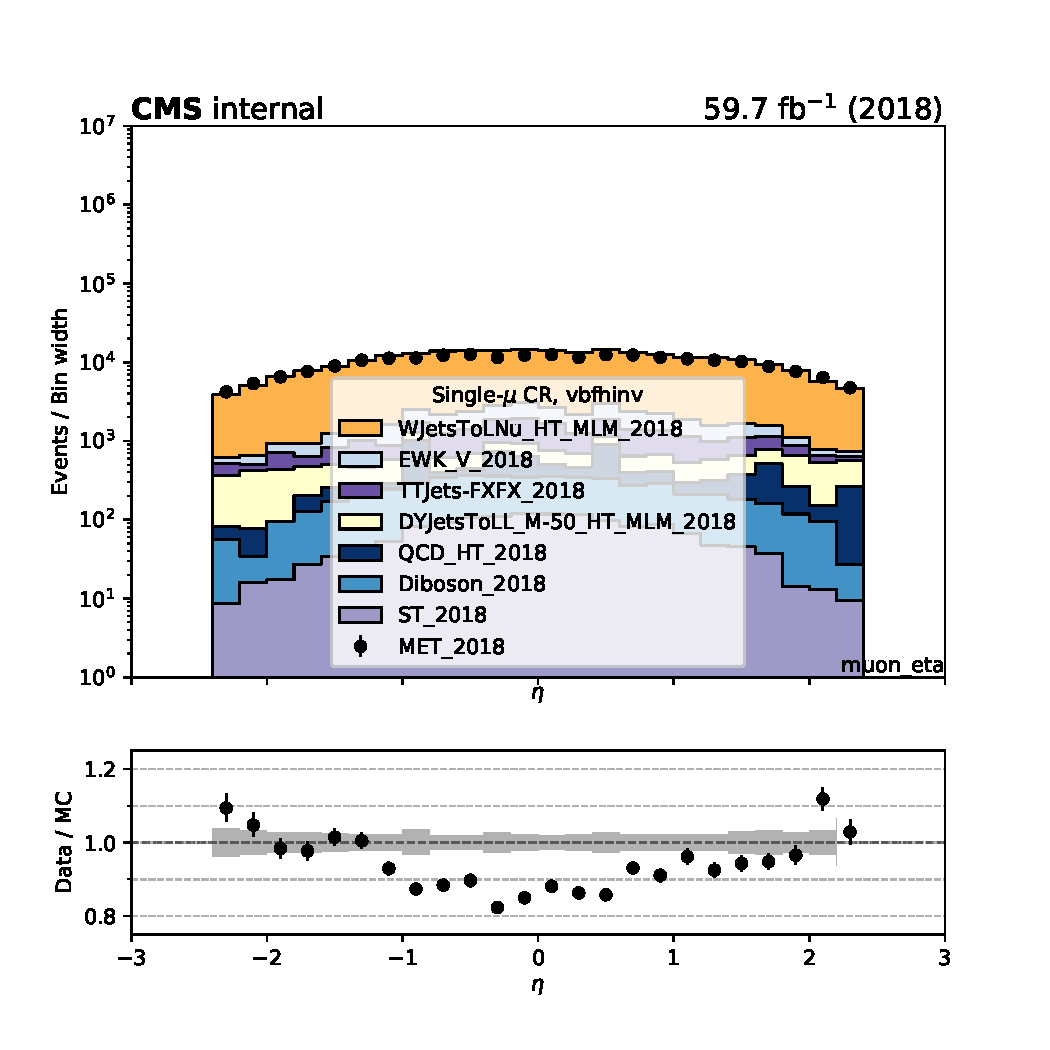
\includegraphics[width=0.49\textwidth]{fig/datamc/cr_1m_vbf/cr_1m_vbf_muon_eta_losf_2018.pdf}
        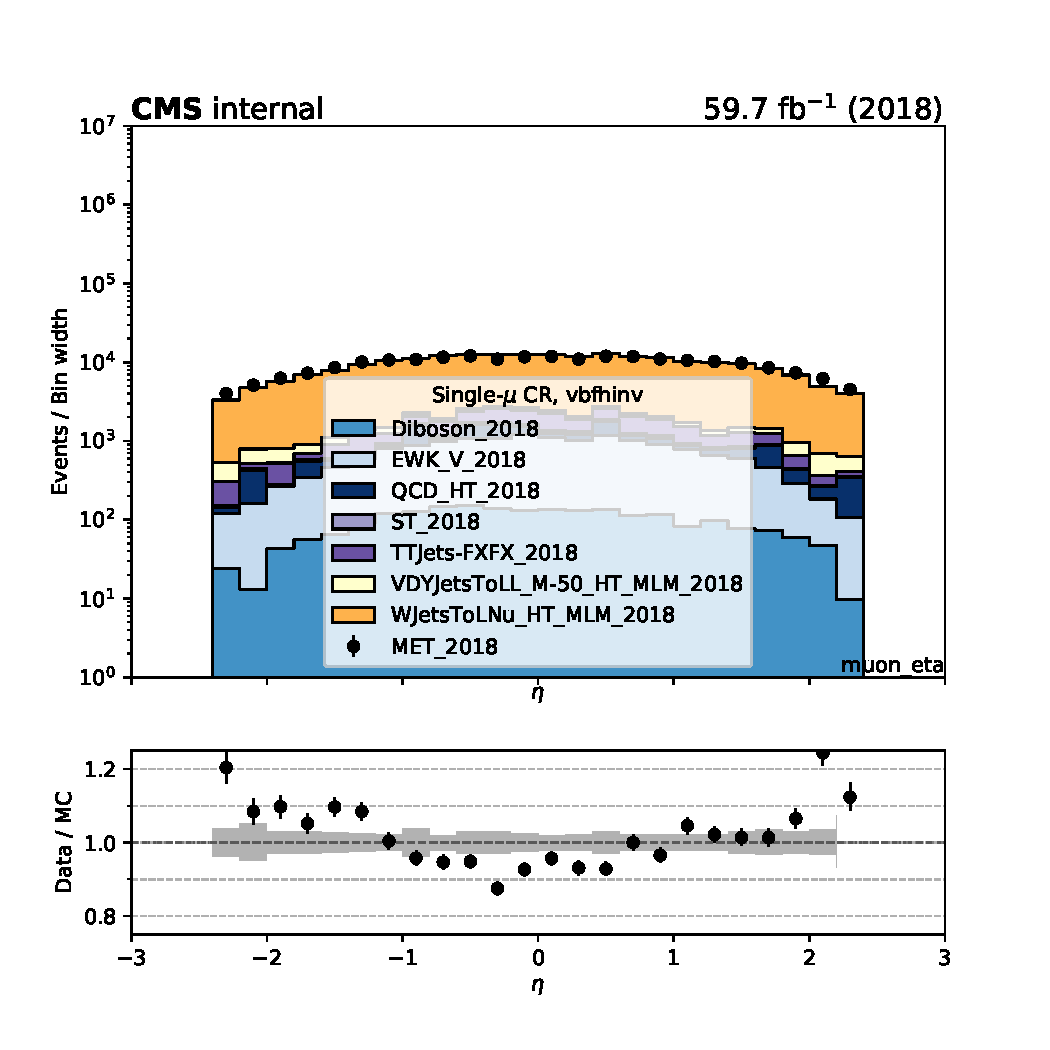
\includegraphics[width=0.49\textwidth]{fig/datamc_2dkfac/cr_1m_vbf/cr_1m_vbf_muon_eta_losf_2018.pdf} 
        \caption{The muon $\eta$ distribution in the single muon CR for the case in which 1D k-factors are used (left), 
        compared to the case in which 2D k-factors are used (right), using 2018 samples.}
        \label{fig:muon_eta_2018}
    \end{center}
\end{figure}